% !TEX root = ../notes.tex

% ================  Unsupervised Learning ==============

\section{Handling Text}

Again, this section has not ambition to explicit all text handling methods but to give an overview of what are the difficulties encountered in this field.
% reorganize the notes by chapter: Handling Data, Text, Images and Graph ??

Information Retrieval (IR) is \textbf{finding material} (usually documents) of an \textbf{unstructured nature} (usually text) that satisfies an \textbf{information need} from within \textbf{large collections} (usually stored on computers).

We name {\bf collection} or {\bf corpus} a set of documents

\begin{figure}[H]%---------------FIG--------------
 \centering
 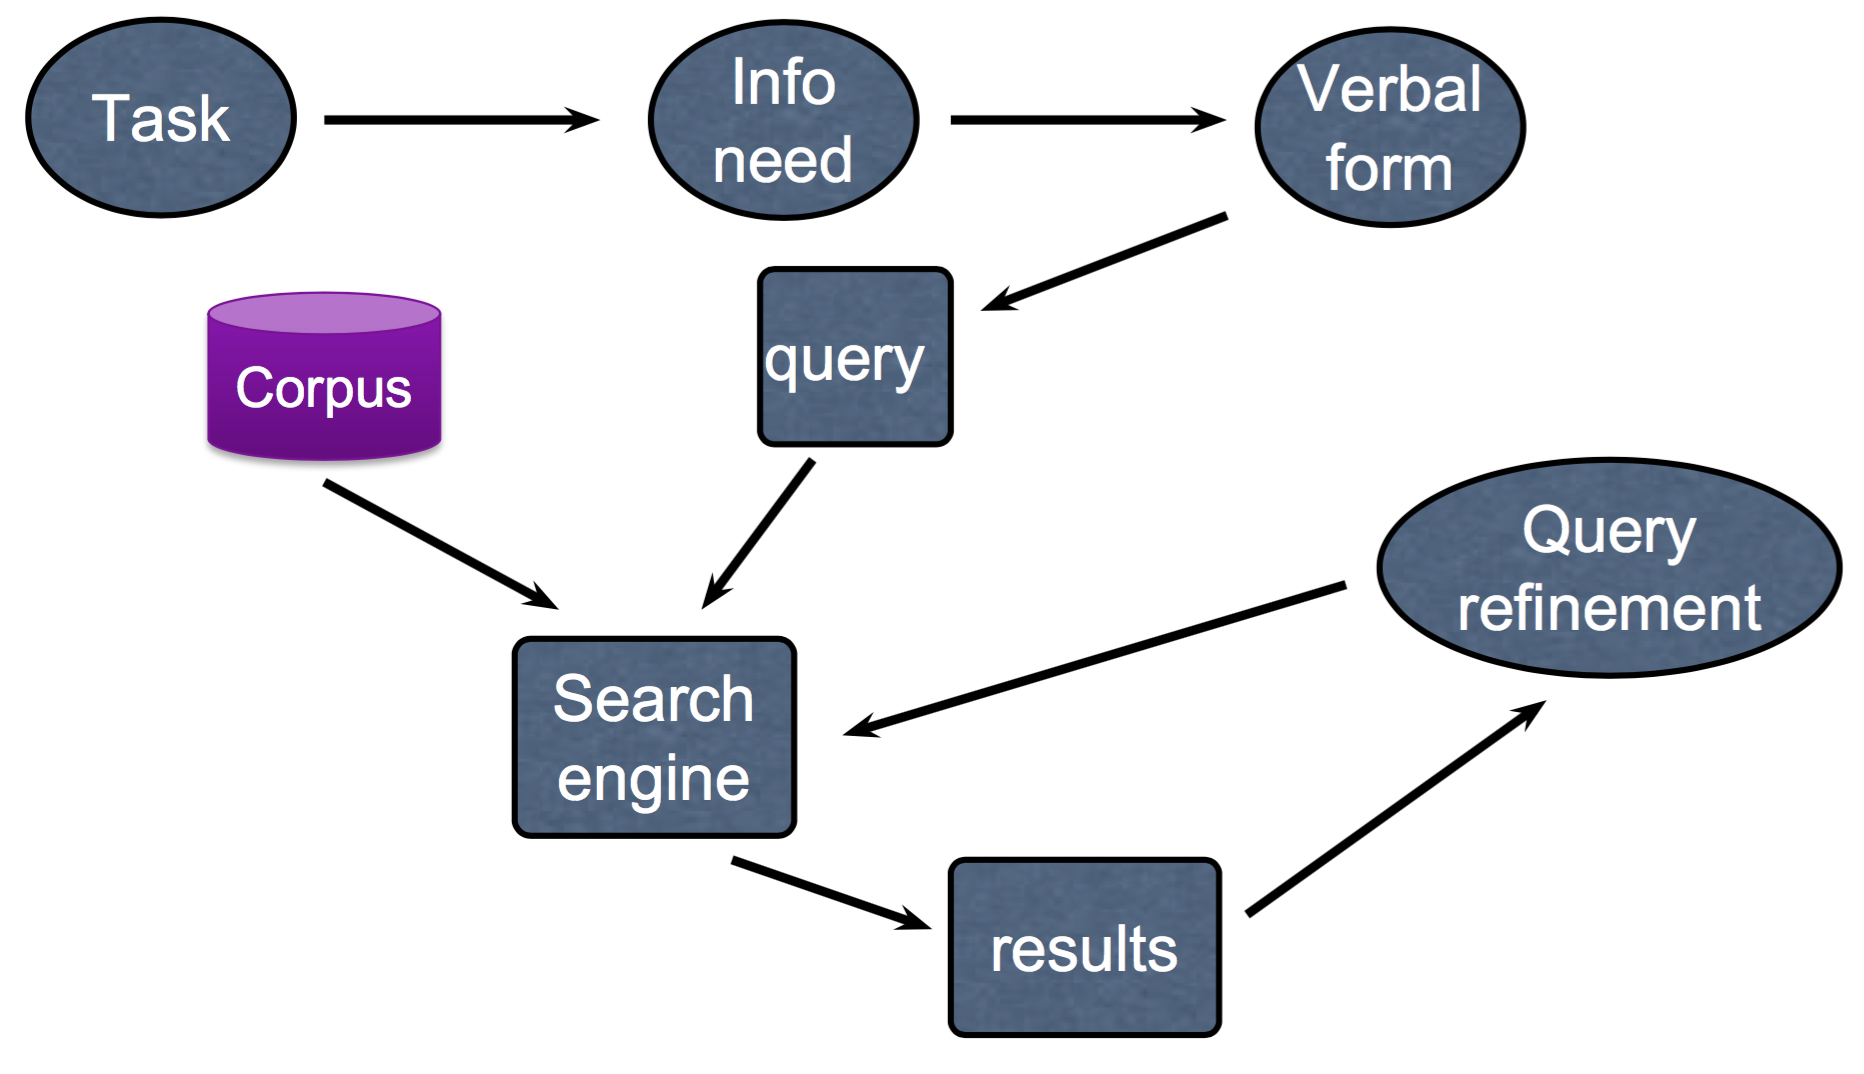
\includegraphics[width=13cm]{./img/11/SE_pipeline}
 \caption{\label{pic:SE_pipline} Search engines pipeline.}
\end{figure}

\subsection{Types of Search Engines}

\begin{itemize}
	\item Q\&A engines
	\item Collaborative
	\item Enterprise
	\item Web
	\item Metasearch
	\item Semantic
	\item NLP
	\item ...
\end{itemize}


\subsection{Challenges of Information Retrieval}

Important thing to always remember when dealing with information retrieval is that the main bottleneck is due to {\bf human cognition} and not computational problem. People often have very unclear definition of concepts, even of very common ones, and they can often disagree between them.

\subsubsection{Queries}

Queries are (or can be) often submitted by users who do not know how works search engines and can not help them to clarify ambiguities. Also, some users do not even know what they want to retrieve or how to name it.

\subsubsection{The concept of {\it relevance}}

Search engines try to retrieve {\bf relevant} documents according with user queries. But a intrinsic problem it to define {\bf what is relevant} because it changes from one user to an other. Is relevance about usefulness? Novelties ? Interest? All of them?

At the end, only real people can judge efficiency of a search engine !

\subsubsection{Representation}

Computers need a way to represent the items contained in their database. How do you represent a documents? An image? A video?

Typically, a document can be represented by a bag-of-words containing the most ones appearing inside it. But that's not enought. Someone can be more interested in meta-data such as date of publication or author.

\subsubsection{Semantic}

Computer can handle words efficiently but, again, it is not sufficient. Meaning of the same word can differ from context to an other, or even from opinion to an other! 

A {\it jaguar} could represent an animal or a car.

A {\it bank} could represent a financial institution, a blood stock or even... a school a fish.

\subsection{Document views}

\begin{itemize}
	\item {\bf Content view} is concerned with representing the content of the document; that is, what is the document about.
	\item {\bf Data view}  is concerned with factual data associated with the document (e.g. author names, publishing date)
	\item {\bf Layout view} is concerned with how documents are displayed to the users; this view is related to user interface and visualization issues.
	\item {\bf Structure view} is concerned with the logical structure of the document, (e.g. a book being composed of chapters, themselves composed of sections, etc.)
\end{itemize}


\subsection{NLP Pipeline}

Here is decribed the pipeline followed when trying to represent a human-written document into a item representable by a computer.

\begin{itemize}
	\item Parsing: Extract information from the document
	\begin{itemize}
		\item regarding format: html, PDF, excel, ... 
		\item character encoding: UFT-8, ...
		\item languages
	\end{itemize}
	
	\item Tokenization: token is an instance of a sequence of characters. All of them will be (after further processing) candidate to be index entry of documents.
	\begin{itemize}
		\item Pair of word going together: Hewlett-Packard must not be split during tokenization
		\item Direction of reading: arabic right to left, but left to right for numbers
		\item Word Separator: Chinese and Japanese have no spaces between words
		\item Alphabet: Japanese uses Katakana, Hiragana, Kani and Romaji alphabet mixture
	\end{itemize}
	
	\item Stop-words list: remove all noisy word using pre-constructed (or enhanced) list.
	\begin{itemize}
		\item english stop-words: and, to, or, the, ...
	\end{itemize}
	
	\item Normalization
	\begin{itemize}
		\item Case folding: reduce to lowercase, but can bring problem. {\it CAT} (acronym of Caterpillar Inc.) must no be mistaken with a {\it cat}.
		\item Accent in French:  {\it r\'esum\'e} or  {\it resume} 
		\item Umlaut in German: {\it Tuebingen} or {\it T\"ubingen}
	\end{itemize}
	
	\item Thesauri and soundex link words with their synonyms 
	\begin{itemize}
		\item by hand-contructing equivalence classes: car = automobile
		\item by expand submited queries: when search for {\it automobile} add it {\it car}
	\end{itemize}
	
	\item Stemming / Lemmatization: normalizes the words to their stem or lemma form.
	\begin{itemize}
		\item Stemming: reduce the the {\it root} by affix chopping (Porter's algorithm): example $\rightarrow$ exampl
		\item Lemmatization: retrieve the cannonical form of each word. More proper than stemming but also more complicated to use because must be based on dictionnary.
	\end{itemize}

\end{itemize}

\begin{figure}[H]%---------------FIG--------------
 \centering
 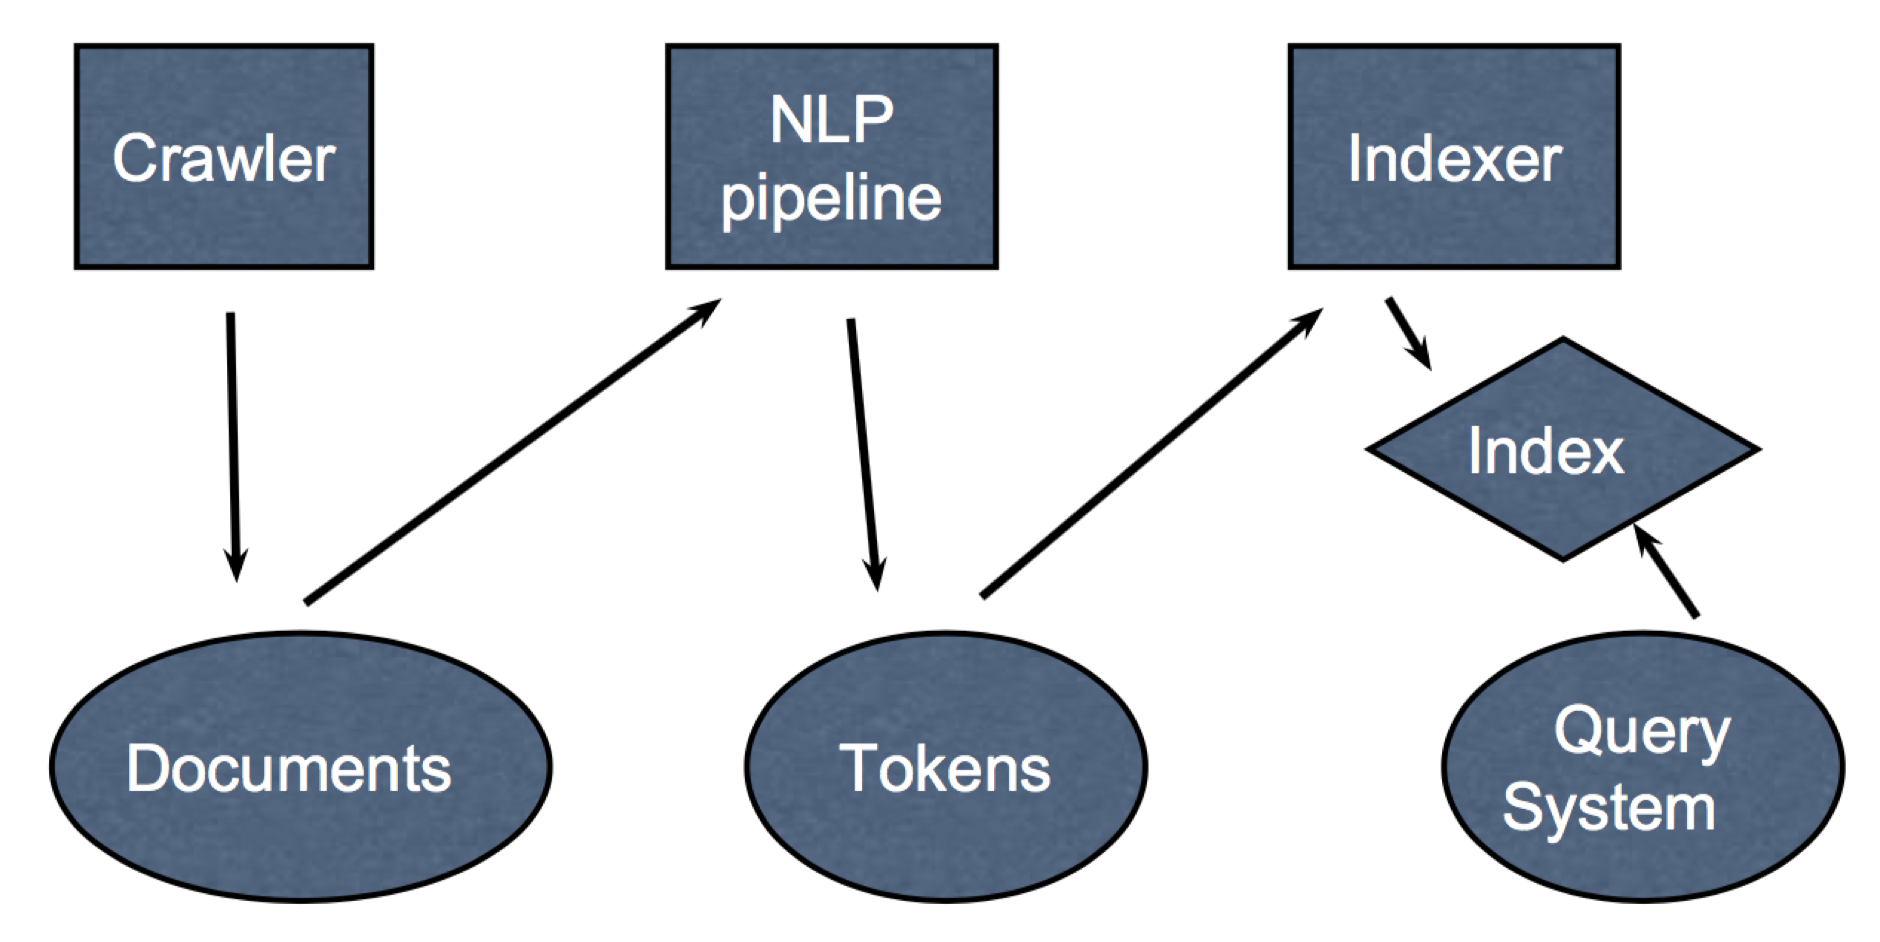
\includegraphics[width=13cm]{./img/11/SE_architecture}
 \caption{\label{pic:SE_pipline} Search engines architecture.}
\end{figure}


% page 63

























